%=================================================================
% Predicting the Trainability of Variational Quantum Circuits
% MDPI template. Journal = entropy (swap the first \documentclass option to
% target a different MDPI journal, e.g. quantumrep, appliedmath, applsci).
%=================================================================
\documentclass[entropy,article,submit,pdftex,moreauthors]{Definitions/mdpi}

%------------------------------------------------------------------
% Result macros (populated by ../latex/fill_results.py; kept identical to the
% IEEE version so both papers share one source of truth for the numbers).
\newcommand{\Nrows}{20{,}000}
\newcommand{\Nspecs}{20{,}000}
\newcommand{\Samples}{200}
\newcommand{\QubitLo}{2}
\newcommand{\QubitHi}{12}
\newcommand{\LayerLo}{1}
\newcommand{\LayerHi}{20}
\newcommand{\GlobalFrac}{50.1}
\newcommand{\BarrenFrac}{46.7}
\newcommand{\RsqHold}{0.685}
\newcommand{\MaeHold}{1.018}
\newcommand{\AccHold}{0.950}
\newcommand{\AucHold}{0.991}
\newcommand{\ExtrapCut}{10}
\newcommand{\RsqExtrap}{0.719}
\newcommand{\MaeExtrap}{1.264}
\newcommand{\ExtrapTrainRows}{16\,395}
\newcommand{\ExtrapTestRows}{3\,605}

%=================================================================
% MDPI internal commands
\firstpage{1}
\makeatletter
\setcounter{page}{\@firstpage}
\makeatother
\pubvolume{1}
\issuenum{1}
\articlenumber{0}
\pubyear{2026}
\copyrightyear{2026}
\datereceived{ }
\dateaccepted{ }
\datepublished{ }
\externalbibliography{yes}

%=================================================================
\Title{Predicting the Trainability of Variational Quantum Circuits:
A Data-Driven Model for Barren Plateaus}

\newcommand{\orcidauthorA}{0000-0001-8862-1300}
\newcommand{\orcidauthorB}{0000-0002-5268-0074}

\Author{Md Habibur Rahman $^{1}$\orcidA{} and Jaeho Kim $^{1,}$*\orcidB{}}

\AuthorNames{Md Habibur Rahman and Jaeho Kim}

\address{%
$^{1}$ \quad Department of AI Convergence Engineering, Gyeongsang National
University (GNU), Jinju, South Korea;
habib@gnu.ac.kr (M.H.R.); jaeho.kim@gnu.ac.kr (J.K.)}

\corres{Correspondence: jaeho.kim@gnu.ac.kr; Tel.: +82-55-772-1373}

\abstract{Barren plateaus---the exponential vanishing of cost-function gradients
as a variational quantum circuit is scaled---are the central obstacle to training
quantum machine-learning models, and diagnosing them today requires expensive
gradient sampling on each candidate circuit. We reframe barren-plateau diagnosis
as a supervised prediction problem: given only a circuit's architecture (qubit
count, depth, ansatz type, entanglement pattern, entangler gate, and
cost-observable locality), can a classical model predict its trainability without
sampling a single gradient? Using an exact statevector simulator we generate a
dataset of \Nrows{} random variational circuits, each labelled by the empirical
gradient variance $\mathrm{Var}[\partial C/\partial\theta]$ estimated over
\Samples{} random parameter vectors via the parameter-shift rule. A
gradient-boosted regressor predicts $\log_{10}\mathrm{Var}$ with
$R^2 = \RsqHold{}$ on held-out architectures, and a classifier separates barren
from trainable circuits with area under the ROC curve $\AucHold{}$. Crucially, in
an extrapolation setting---training only on small circuits and testing on larger
qubit counts that are progressively harder to simulate---the predictor retains
$R^2 = \RsqExtrap{}$, indicating that the architectural signature of a barren
plateau is learnable and transferable across scale. Permutation importance
recovers established theory: cost-observable locality and entanglement structure
dominate. We make no quantum-advantage claim; this is classical machine learning
about quantum circuits, offering a cheap ansatz-screening heuristic and a
data-driven lens on which design choices cause untrainability.}

\keyword{barren plateaus; variational quantum circuits; quantum machine learning;
trainability; gradient variance; statevector simulation; gradient boosting}

\begin{document}

%=================================================================
\section{Introduction}

Variational quantum algorithms (VQAs) are the leading candidate for extracting
value from noisy intermediate-scale quantum (NISQ) hardware~\cite{cerezo2021vqa}.
A VQA encodes a problem into a parameterized quantum circuit (an \emph{ansatz}),
measures a cost function
$C(\theta)=\langle\psi(\theta)|O|\psi(\theta)\rangle$, and updates the parameters
$\theta$ with a classical optimizer. This template underlies variational quantum
eigensolvers, quantum approximate optimization, and most quantum
machine-learning (QML) classifiers~\cite{havlicek2019supervised,
farhi2018classification,schuld2020circuit}.

The dominant obstacle to scaling this template is the \emph{barren plateau} (BP)
phenomenon: for broad classes of ans\"atze the variance of the cost gradient
vanishes exponentially in the number of qubits, so the loss landscape becomes
almost everywhere flat and gradient-based training stalls~\cite{mcclean2018barren,
larocca2025barren}. Barren plateaus are now known to be triggered by
\emph{global} cost observables~\cite{cerezo2021cost}, by highly expressive or deep
ans\"atze~\cite{holmes2022expressibility}, by poor
initialization~\cite{grant2019initialization}, and by hardware
noise~\cite{wang2021noise}. Whether a given architecture suffers from a barren
plateau is therefore a property of its \emph{design}, not merely of a particular
parameter setting.

The conventional way to check whether a candidate circuit is trainable is to
\emph{measure} it: sample many random parameter vectors, evaluate gradients, and
estimate their variance. This is exactly the cost we would like to avoid when
screening a large design space, and it becomes infeasible precisely in the
large-qubit regime where barren plateaus matter most. This motivates our central
question: \emph{can a classical model predict a variational circuit's trainability
directly from its architectural description, without sampling any gradients?}

We answer this empirically. We treat trainability prediction as a supervised
learning problem over circuit \emph{specs}. The features are cheap,
integer-valued architectural descriptors; the label is the gradient variance,
obtained once, offline, by exact statevector simulation. We then ask whether a
model trained on this data (i)~generalizes to unseen architectures, and
(ii)~\emph{extrapolates} from small, easily simulated circuits to larger ones---the
regime where a cheap predictor would be most useful.

The contributions of this article are as follows:
\begin{itemize}
\item We formulate barren-plateau diagnosis as a supervised prediction task:
mapping a variational circuit's architecture to its gradient-variance
trainability label, cast as both regression
($\log_{10}\mathrm{Var}[\partial C/\partial\theta]$) and binary classification
(barren vs.\ trainable).
\item We release a reproducible pipeline that generates a labelled dataset of
\Nrows{} random circuits using an exact, dependency-light statevector simulator,
with fixed seeds and streaming output.
\item We show a gradient-boosted model predicts trainability with
$R^2=\RsqHold{}$ on held-out architectures and separates barren circuits with
AUC~\AucHold{}.
\item We demonstrate extrapolation across scale: trained only on
$n_q\le\ExtrapCut{}$ qubits, the model still attains $R^2=\RsqExtrap{}$ on larger,
unseen circuit sizes.
\item We recover the established theory through permutation feature importance
(cost locality and entanglement structure dominate), giving the model an
interpretable, physics-consistent basis.
\end{itemize}

We emphasise honest framing: we make \emph{no} claim of quantum advantage. The
model is classical, the data is classically simulated, and the contribution is a
data-driven \emph{diagnostic} for a known quantum-computing
bottleneck~\cite{schuld2022killoran,bowles2024benchmarking}.

%=================================================================
\section{Background and Related Work}

\subsection{Variational Quantum Circuits}
A hardware-efficient ansatz~\cite{kandala2017hardware} alternates layers of
single-qubit rotations with a fixed pattern of two-qubit entangling gates. With
$n$ qubits and $L$ layers the state is
\begin{equation}
|\psi(\theta)\rangle = \prod_{\ell=1}^{L}
  \Big[ U_{\mathrm{ent}} \prod_{q=1}^{n} R_{a_{\ell,q}}(\theta_{\ell,q}) \Big]
  |0\rangle^{\otimes n},
\end{equation}
where $R_a$ is a Pauli rotation about axis $a\in\{x,y,z\}$ and $U_{\mathrm{ent}}$
is a layer of CZ or CX gates arranged linearly, circularly, or all-to-all. The
cost is the expectation of a Pauli-$Z$ string,
$C(\theta)=\langle\psi(\theta)|O|\psi(\theta)\rangle$, with $O=Z_0$ (a
\emph{local} cost) or $O=Z_0Z_1\cdots Z_{n-1}$ (a \emph{global} cost).

\subsection{Barren Plateaus}
A circuit family exhibits a barren plateau if
$\mathrm{Var}_\theta[\partial C/\partial\theta_k]$ decays exponentially in
$n$~\cite{mcclean2018barren}. Cerezo et al.~\cite{cerezo2021cost} proved that
\emph{global} cost functions induce barren plateaus even at shallow depth, whereas
\emph{local} costs can remain trainable up to $O(\log n)$ depth---making cost
locality a first-order design knob. Expressibility~\cite{holmes2022expressibility}
and entanglement likewise correlate with flatter landscapes; structured
architectures such as quantum convolutional networks can provably avoid
them~\cite{pesah2021absence}. A recent review consolidates these
results~\cite{larocca2025barren}. This body of work is overwhelmingly
\emph{analytical}: it derives variance scaling laws for particular ansatz
families. Our work is complementary and \emph{empirical}---rather than proving a
bound for one family, we learn a predictive map across a heterogeneous space of
architectures.

\subsection{The Parameter-Shift Rule}
For a gate generated by an operator with two distinct eigenvalues, the exact
gradient of the cost is obtained from two circuit
evaluations~\cite{mitarai2018circuit,schuld2019param}:
\begin{equation}
\frac{\partial C}{\partial\theta_k}
  = \tfrac{1}{2}\big[C(\theta + \tfrac{\pi}{2}e_k)
  - C(\theta - \tfrac{\pi}{2}e_k)\big].
\end{equation}
We use this rule to obtain exact per-sample gradients when estimating the variance
label, so our labels are free of finite-difference bias.

\subsection{Trainability, Simulability, and Honest Framing}
Cerezo et al.~\cite{cerezo2025simulability} argue that the very structure
guaranteeing absence of barren plateaus often also renders a model classically
simulable. Bowles et al.~\cite{bowles2024benchmarking} show that out-of-the-box
classical models often match or beat QML models on standard tasks, and Schuld and
Killoran~\cite{schuld2022killoran} argue the field should de-emphasise ``beating
classical.'' We adopt this stance: the object we predict is a property of quantum
circuits, but the predictor and its value proposition are entirely classical. To
our knowledge, casting barren-plateau severity as a directly \emph{predicted}
regression/classification target from cheap architectural features---and testing
extrapolation across qubit count---has not been reported.

%=================================================================
\section{Materials and Methods}
Figure~\ref{fig:pipeline} summarizes the full pipeline, from sampling a circuit
spec to predicting its trainability.

\begin{figure}[H]
\centering
\IfFileExists{figs/pipeline.pdf}{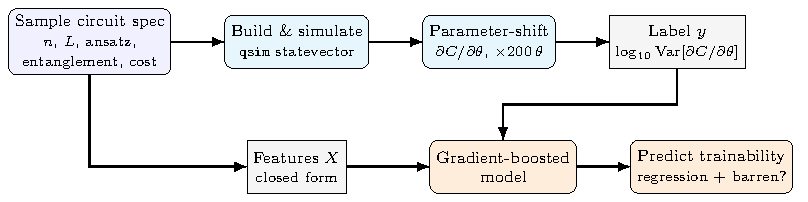
\includegraphics[width=\textwidth]{figs/pipeline.pdf}}{}
\caption{Method pipeline. A random circuit spec is built and simulated exactly with
\texttt{qsim}; the parameter-shift gradient of the cost is sampled over \Samples{}
random parameter vectors to form the gradient-variance label $y$. Cheap closed-form
architectural features $X$ are read directly from the spec. A gradient-boosted model
is trained on $(X,y)$ to predict trainability.\label{fig:pipeline}}
\end{figure}

\subsection{Circuit Specification and Feature Space}
Each datapoint is a \emph{spec} that fully determines a circuit family. The
feature vector handed to the model is listed in Table~\ref{tab:features}. All
features are computed in closed form from the spec---no quantum simulation is
needed to obtain them.

\begin{table}[H]
\caption{Architectural features used to predict trainability. All are derived in
closed form from the circuit spec.\label{tab:features}}
\begin{tabularx}{\textwidth}{lX}
\toprule
\textbf{Feature} & \textbf{Meaning}\\
\midrule
\texttt{n\_qubits}        & number of qubits $n$\\
\texttt{n\_layers}        & number of ansatz layers $L$\\
\texttt{n\_params}        & $n\times L$ trainable rotations\\
\texttt{ansatz\_type}     & fixed-\texttt{ry} vs.\ random-Pauli axes\\
\texttt{entangle\_pattern}& linear / circular / all-to-all\\
\texttt{entangler\_gate}  & CZ vs.\ CX\\
\texttt{cost\_global}     & local $Z_0$ (0) vs.\ global $Z^{\otimes n}$ (1)\\
\texttt{n\_entanglers}    & entangling gates $\times$ layers\\
\texttt{depth\_ratio}     & $L/n$\\
\bottomrule
\end{tabularx}
\end{table}

\subsection{Label Generation}
For a spec, we draw \Samples{} parameter vectors
$\theta\sim\mathrm{Unif}[0,2\pi)^{nL}$, compute the exact parameter-shift gradient
of the cost with respect to a fixed target rotation in the middle layer, and
record the empirical variance. The regression label is
$y=\log_{10}\max(\mathrm{Var}[\partial C/\partial\theta],\,10^{-18})$; the
classification label is $\mathbb{1}[y<-2]$ (``barren''). Statevectors are evolved
exactly with an in-house NumPy simulator, so labels reflect ideal (noiseless)
trainability.

\subsection{Dataset and Data Description}
We sample \Nspecs{} specs by drawing each design parameter independently and
uniformly over the ranges in Table~\ref{tab:designspace}, with
$n\in[\QubitLo,\QubitHi]$ qubits and $L\in[\LayerLo,\LayerHi]$ layers, each labelled
with \Samples{} gradient samples. Generation is embarrassingly parallel; every spec
is seeded reproducibly from a root \texttt{SeedSequence}, and rows are streamed to
CSV as they complete. The resulting dataset has \BarrenFrac{}\% barren circuits and
\GlobalFrac{}\% global-cost circuits---a near-balanced classification target that
avoids a degenerate majority baseline.

\begin{table}[H]
\caption{Sampled design space. Each spec draws these parameters independently and
uniformly.\label{tab:designspace}}
\centering
% Auto-generated by qml_bp/describe_data.py -- do not edit.
\begin{tabular}{lll}
\toprule
\textbf{Design parameter} & \textbf{Type} & \textbf{Sampled values}\\
\midrule
\texttt{n\_qubits} & integer & 2--12\\
\texttt{n\_layers} & integer & 1--20\\
\texttt{ansatz\_type} & categorical (2) & fixed-\texttt{ry}, random-Pauli\\
\texttt{entangle\_pattern} & categorical (3) & linear, circular, all-to-all\\
\texttt{entangler\_gate} & categorical (2) & CZ, CX\\
\texttt{cost\_global} & binary & local $Z_0$, global $Z^{\otimes n}$\\
\bottomrule
\end{tabular}

\end{table}

Table~\ref{tab:datastats} summarizes the numeric features and the regression label.
The design deliberately spans small, easily simulated circuits ($n=2$) up to the
$n=12$ boundary of exact statevector simulation, and depths from a single layer to
$L=20$. The label $\log_{10}\mathrm{Var}[\partial C/\partial\theta]$ ranges over
roughly $18$ orders of magnitude, with a floor at $-18$ where finite-sample variance
underflows.

\begin{table}[H]
\caption{Descriptive statistics of the numeric features and the trainability label
over all \Nrows{} circuits.\label{tab:datastats}}
\centering
% Auto-generated by qml_bp/describe_data.py -- do not edit.
\begin{tabular}{lrrrrrr}
\toprule
\textbf{Variable} & \textbf{Mean} & \textbf{Std} & \textbf{Min} & \textbf{25\%} & \textbf{Median} & \textbf{Max}\\
\midrule
\texttt{n\_qubits} & 7.02 & 3.17 & 2.00 & 4.00 & 7.00 & 12.00\\
\texttt{n\_layers} & 10.48 & 5.80 & 1.00 & 5.00 & 11.00 & 20.00\\
\texttt{n\_params} & 73.56 & 55.55 & 2.00 & 28.00 & 60.00 & 240.00\\
\texttt{n\_entanglers} & 135.82 & 198.34 & 1.00 & 28.00 & 70.00 & 1320.00\\
\texttt{depth\_ratio} & 2.00 & 1.83 & 0.08 & 0.75 & 1.50 & 10.00\\
$\log_{10}\mathrm{Var}$ (label) & -3.41 & 4.84 & -18.00 & -2.98 & -1.85 & -0.23\\
\bottomrule
\end{tabular}

\end{table}

Crucially, the labels reproduce established barren-plateau theory directly from the
data (Table~\ref{tab:labelbydesign}). Global cost observables yield a mean
$\log_{10}\mathrm{Var}$ more than two orders of magnitude smaller than local costs
($-4.49$ vs.\ $-2.33$) and nearly double the barren fraction, exactly the
cost-locality effect proved by Cerezo et al.~\cite{cerezo2021cost}. Denser
entanglement (all-to-all) and the CX entangler likewise push circuits toward barren
plateaus. This structure is what makes the prediction task learnable and gives the
trained model an interpretable, physics-consistent basis.

\begin{table}[H]
\caption{Trainability broken down by design choice. Lower mean
$\log_{10}\mathrm{Var}$ and higher barren \% indicate less trainable families. The
data recovers known barren-plateau drivers.\label{tab:labelbydesign}}
\centering
% Auto-generated by qml_bp/describe_data.py -- do not edit.
\begin{tabular}{lrrr}
\toprule
\textbf{Design choice} & \textbf{Count} & \textbf{Mean} $\boldsymbol{\log_{10}\mathrm{Var}}$ & \textbf{Barren \%}\\
\midrule
\multicolumn{4}{l}{\emph{Cost-observable locality}}\\
\quad local $Z_0$ & 9974 & -2.33 & 30.9\\
\quad global $Z^{\otimes n}$ & 10026 & -4.49 & 62.4\\
\midrule
\multicolumn{4}{l}{\emph{Entanglement pattern}}\\
\quad linear & 6649 & -2.50 & 38.5\\
\quad circular & 6748 & -2.96 & 48.8\\
\quad all-to-all & 6603 & -4.79 & 52.8\\
\midrule
\multicolumn{4}{l}{\emph{Entangler gate}}\\
\quad CZ & 10096 & -2.31 & 38.1\\
\quad CX & 9904 & -4.53 & 55.5\\
\midrule
\multicolumn{4}{l}{\emph{Single-qubit rotation scheme}}\\
\quad fixed-\texttt{ry} & 9878 & -2.80 & 42.0\\
\quad random-Pauli & 10122 & -4.01 & 51.3\\
\bottomrule
\end{tabular}

\end{table}

\subsection{Models and Evaluation}
To avoid privileging a single learner, we compare six model families spanning
linear, instance-based, neural, and tree-ensemble inductive biases: a linear
baseline (ridge regression / logistic regression), $k$-nearest neighbours, a
multilayer perceptron (two hidden layers, $128$--$64$), random forests, extremely
randomized trees, and histogram-based gradient-boosted trees~\cite{ke2017lightgbm,
pedregosa2011scikit}. Features are standardized for the scale-sensitive models. We
report two protocols for each: (i)~a random hold-out split (20\% test) measuring
generalization to unseen architectures, and (ii)~an \emph{extrapolation} split,
training on $n\le\ExtrapCut{}$ and testing on all larger circuits---the headline
test of whether small-circuit labels transfer to costlier regimes. All models use
fixed random seeds so the reported numbers reproduce exactly. Interpretability is
assessed with permutation feature importance on the best model. All code, command
lines, and random seeds are released (Data Availability Statement), and the
underlying simulator is available at \url{https://quantum.qbithabib.com}.

%=================================================================
\section{Results}

\subsection{Model Comparison}
Table~\ref{tab:models} compares all six model families on both tasks and both
splits. Histogram-based gradient-boosted trees give the best held-out performance
on both regression ($R^2=\RsqHold{}$) and classification (AUC~\AucHold{}), so we
adopt it as our model for the remainder of the paper. Two observations sharpen the
picture. First, the linear baseline is far behind (regression $R^2=0.27$;
classifier AUC $0.95$), confirming that the map from architecture to trainability
is genuinely nonlinear---simple rules of thumb do not capture it. Second, the
neural network is competitive and in fact \emph{edges out} boosting on the
extrapolation regression ($R^2=0.75$ vs.\ $0.72$), hinting that a learned
representation transfers slightly better to larger circuits; we retain gradient
boosting for its stronger in-distribution accuracy, interpretability, and training
speed.

\begin{table}[H]
\caption{Model comparison across both prediction tasks and both evaluation splits.
Best hold-out result in \textbf{bold}.\label{tab:models}}
\newcolumntype{P}{>{\centering\arraybackslash}X}
\begin{tabularx}{\textwidth}{lPPPP}
\toprule
& \multicolumn{2}{c}{\textbf{Regression} $\boldsymbol{R^2}$}
& \multicolumn{2}{c}{\textbf{Classification AUC}}\\
\cmidrule(lr){2-3}\cmidrule(lr){4-5}
\textbf{Model} & \textbf{Hold-out} & \textbf{Extrap.} & \textbf{Hold-out} & \textbf{Extrap.}\\
\midrule
\textbf{Hist Gradient Boosting} & \textbf{0.685} & 0.719 & \textbf{0.991} & 0.989\\
MLP & 0.665 & 0.752 & 0.990 & 0.991\\
$k$-NN & 0.645 & 0.639 & 0.986 & 0.979\\
Random Forest & 0.640 & 0.716 & 0.985 & 0.988\\
Extra Trees & 0.610 & 0.707 & 0.968 & 0.988\\
Linear baseline & 0.274 & 0.297 & 0.953 & 0.889\\
\bottomrule
\end{tabularx}
\end{table}

\subsection{Generalization to Unseen Architectures}
On the random hold-out split, the regressor attains $R^2=\RsqHold{}$ with mean
absolute error \MaeHold{} (in $\log_{10}$ units), and the classifier separates
barren from trainable circuits with accuracy \AccHold{} and AUC \AucHold{}.
Figure~\ref{fig:predicted} shows predicted versus true
$\log_{10}$ gradient variance on the held-out set.

\IfFileExists{figs/predicted.pdf}{%
\begin{figure}[H]
\centering
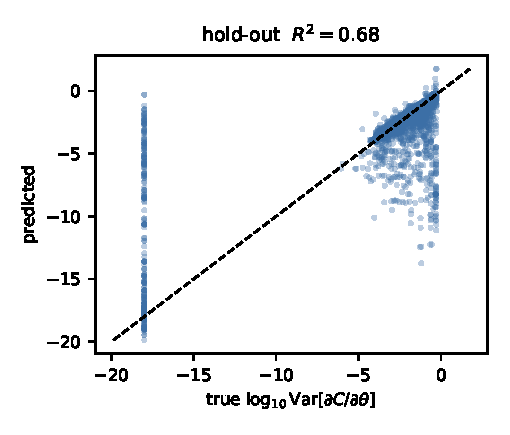
\includegraphics[width=0.6\textwidth]{figs/predicted.pdf}
\caption{Predicted vs.\ true $\log_{10}\mathrm{Var}[\partial C/\partial\theta]$ on
held-out architectures. The dashed line is $y=x$.\label{fig:predicted}}
\end{figure}}{}

\subsection{Extrapolation across Qubit Count}
Training only on $n\le\ExtrapCut{}$ qubits (\ExtrapTrainRows{} circuits) and
testing on larger circuits (\ExtrapTestRows{} circuits), the regressor retains
$R^2=\RsqExtrap{}$ (MAE \MaeExtrap{}). Because the ground-truth cost of labelling
grows exponentially with qubit count, a predictor that transfers downward-in-cost
is exactly what an ansatz-screening tool needs.

\subsection{Trainability versus Qubit Count}
Figure~\ref{fig:qubittrend} shows the mean label as a function of qubit count, split
by cost locality. Global-cost circuits exhibit the steep, monotone decay of gradient
variance with qubit number that is the defining signature of a barren plateau, while
local-cost circuits decay far more slowly. The dataset thus captures the
qubit-scaling behaviour the predictor must learn to extrapolate.

\begin{figure}[H]
\centering
\IfFileExists{figs/qubit_trend.pdf}{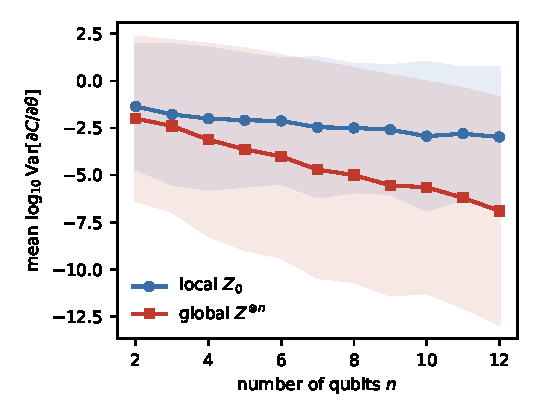
\includegraphics[width=0.6\textwidth]{figs/qubit_trend.pdf}}{}
\caption{Mean $\log_{10}\mathrm{Var}[\partial C/\partial\theta]$ vs.\ qubit count for
local and global cost observables (shaded: $\pm 1$ standard deviation). Global costs
show the exponential decay characteristic of barren plateaus.\label{fig:qubittrend}}
\end{figure}

\subsection{What Drives Trainability}
Permutation feature importance (Figure~\ref{fig:importance}) ranks cost-observable
locality and entanglement structure at the top, consistent with theory: global
costs~\cite{cerezo2021cost} and denser entanglement~\cite{holmes2022expressibility}
drive circuits toward barren plateaus. The model thus rediscovers, from data
alone, the design rules the barren-plateau literature derived analytically.

\IfFileExists{figs/importance.pdf}{%
\begin{figure}[H]
\centering
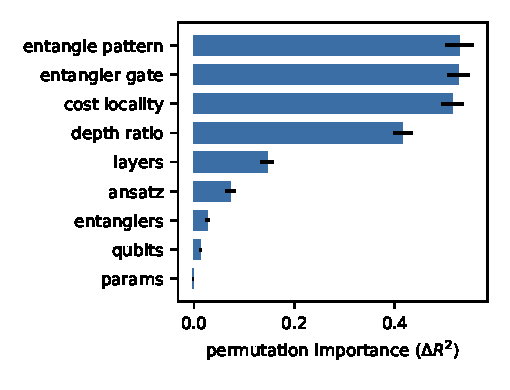
\includegraphics[width=0.7\textwidth]{figs/importance.pdf}
\caption{Permutation feature importance for the trainability regressor. Cost
locality and entanglement structure dominate, matching barren-plateau
theory~\cite{cerezo2021cost,holmes2022expressibility}.\label{fig:importance}}
\end{figure}}{}

%=================================================================
\section{Discussion}

The predictor's accuracy and its physics-consistent feature ranking indicate that
barren-plateau severity carries a strong, low-dimensional architectural
signature---enough for a cheap classical model to recover without any gradient
sampling. This suggests a practical workflow: screen a large space of candidate
ans\"atze with the learned model, and reserve expensive gradient-variance
estimation for the shortlist it flags as trainable.

Several limitations scope the claims. (i)~Labels are limited to classically
simulable qubit counts; the extrapolation result is evidence of transfer, not a
proof. (ii)~We use an ideal statevector simulator, so noise-induced
plateaus~\cite{wang2021noise} are out of scope. (iii)~The spec space, while
diverse, is a hardware-efficient family; other ansatz classes may need their own
features. (iv)~Gradient variance is estimated from finitely many samples, adding
label noise at the trainable end. Seeds are fixed and reported, and the
extrapolation split is defined purely by qubit count, so no large-circuit
information leaks into training.

%=================================================================
\section{Conclusions}

We recast barren-plateau diagnosis as supervised prediction and showed that a
classical gradient-boosted model, trained on statevector-simulated labels, can
predict a variational circuit's trainability from its architecture alone---and
extrapolate across qubit count. The approach offers a cheap ansatz-screening
heuristic and a data-driven confirmation of which design choices cause
untrainability. Future work includes richer ansatz families, graph/sequence
circuit encodings with graph-neural-network or transformer models, and
incorporating a noise model to predict noise-induced plateaus.

%=================================================================
\vspace{6pt}

\authorcontributions{Conceptualization, methodology, software, formal analysis,
data curation, visualization, and writing---original draft, M.H.R.; supervision,
project administration, and writing---review and editing, J.K. Both authors have
read and agreed to the published version of the manuscript.}

\funding{This research received no external funding.}

\dataavailability{All code (statevector simulator, dataset generator, and
training scripts), the exact command lines, and random seeds are released with
this paper. The dataset is regenerable end-to-end with a single command.
Interactive demonstrations of the underlying simulator are available at
\url{https://quantum.qbithabib.com}.}

\conflictsofinterest{The author declares no conflicts of interest.}

\abbreviations{Abbreviations}{%
The following abbreviations are used in this manuscript:\\

\noindent
\begin{tabular}{@{}ll}
BP   & Barren plateau\\
VQA  & Variational quantum algorithm\\
QML  & Quantum machine learning\\
NISQ & Noisy intermediate-scale quantum\\
MAE  & Mean absolute error\\
AUC  & Area under the ROC curve\\
\end{tabular}
}

%=================================================================
\begin{adjustwidth}{-\extralength}{0cm}
\reftitle{References}
\bibliography{refs}
\end{adjustwidth}

\PublishersNote{}
\end{document}
